\documentclass[10pt,executivepaper]{article}
\usepackage[utf8]{inputenc}
\usepackage[spanish]{babel}
\usepackage{amsmath}
\usepackage{amsfonts}
\usepackage{amssymb}
\usepackage{graphics}
\usepackage{graphicx}
\usepackage[left=2cm,right=2cm,top=2cm,bottom=2cm]{geometry}
\usepackage{imakeidx}
\makeindex[columns=3, title=Alphabetical Index, intoc]
\usepackage{listings}
\usepackage{xcolor}
\usepackage{multicol}
\usepackage{changepage}
\usepackage{float}
\usepackage{cite}
\usepackage{url}
\usepackage{lscape}

\definecolor{codegreen}{rgb}{0,0.6,0}
\definecolor{codegray}{rgb}{0.5,0.5,0.5}
\definecolor{codepurple}{rgb}{0.58,0,0.82}
\definecolor{backcolour}{rgb}{0.95,0.95,0.92}

\lstdefinestyle{mystyle}{
    backgroundcolor=\color{backcolour},
    commentstyle=\color{codegreen},
    keywordstyle=\color{magenta},
    numberstyle=\tiny\color{codegray},
    stringstyle=\color{codepurple},
    basicstyle=\ttfamily\footnotesize,
    breakatwhitespace=false,
    breaklines=true,
    captionpos=b,
    keepspaces=true,
    numbers=left,
    numbersep=5pt,
    showspaces=false,
    showstringspaces=false,
    showtabs=false,
    tabsize=3
}

\lstset{style=mystyle}

\title{Actividad: Uso eficiente de la memoria cache}

\author{Instituto Politécnico Nacional\\Escuela Superior de Computo\\Desarrollo de Sistemas Distribuidos\\Adrian González Pardo\\4CV1\\21/01}
\date{\today}
\newcommand\tab[1][1cm]{\hspace*{#1}}

\begin{document}
\maketitle
\section{Código fuente:}
\begin{center}
  \lstinputlisting[language=Java]{../MultiplicaMatriz.java}
  \textit{En este código fuente podemos ver que las operacionel calculo de una matriz de $NxN$ es o puede ser cálculada por las propiedades matemáticas las cuales son $\Sigma(fila\;x\;columna)$ la cual da lugar al cálculo de la matriz el cual puede tener una complejiad $O(N^3)$}
  \lstinputlisting[language=Java]{../MultiplicaMatriz2.java}
  \textit{En este código fuente podemos ver que las operacionel calculo de una matriz de $NxN$ es o puede ser cálculada por las propiedades matemáticas las cuales son $\Sigma(fila\;x\;columna)$ pero con una ligera modificación al código donde podemos ver que se genera una matriz transpuesta $M^T$ de la matriz $B$ por el cual es muy sencillo el acceso de la variable ya que no hay un movimiento $fila\;x\;columna$ sino que su acceso es $fila\;x\;fila$, por ello esta implementación es más eficiente en tiempo.}
\end{center}
\section{Gráfica de ejecución}
\begin{center}
  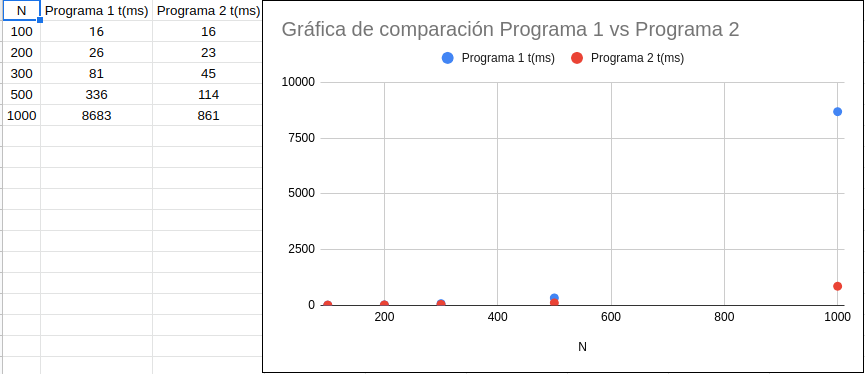
\includegraphics[scale=0.5]{imgs/grafica.png}
  \\\textit{Gráfica de descripción de la ejecución del programa.}
\end{center}
\section{Especificaciones del equipo que lo ejecuto}
\begin{itemize}
  \item Procesador Intel Core I5-3210M CPU 2.50GHz x 2 nucleos físicos (1 nucleo virtual por nucleo)
  \item 3 MB Intel Smart Cache
  \item 12 GB de RAM
\end{itemize}


\end{document}
